\chapter{Assignments}\label{ch:assignments}

\section{Tune your own antenna}
In this section, you'll be customizing your own antenna. Begin by attaching the \gls{sma} connector to the provided patch antenna under the guidance of the lab instructor (see first procedure). Once this is completed, carefully trim small sections from the corners to fine-tune the antenna for operation at \SI{917}{\mega\hertz}.\footnote{Why don't we buy a ready-made antenna? The answer is sustainability and learning by experience. The antennas used in this lab session were manufactured with the wrong substrate altering the expected specifications of the antenna, i.e., it is de-tuned from it's designed frequency. Rather than throwing them in the bin, we reuse them in this lab. Similarly, the \gls{sma} connectors had to be altered before use.}

Procedure connector:
\begin{enumerate}
    \item Remove the excess coating on the feed pin of the \gls{sma} connector with a cutter knife. \textbf{Before beginning, seek additional details from your lab instructor on the cutting process. Additionally, exercise caution as sharp tools are involved—cut away from the body (and fingers).}
    \item Enlarge the hole of the feed point of the antenna by drilling (\SI{1.5}{mm}).
    \item Solder the connector on the antenna, two ground planes of the connector and the feed point at the front of the antenna. See~\cref{fig:patch}.
\end{enumerate}

\begin{figure}[hbtp]
    \centering
    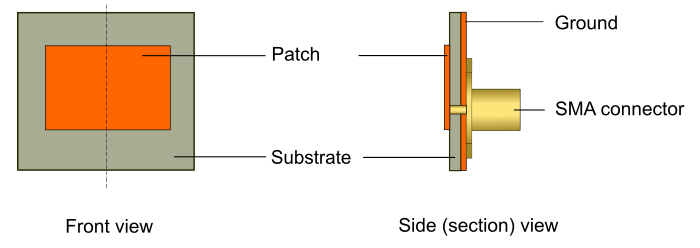
\includegraphics[width=0.8\linewidth]{figs/patch_microstrip_pin_fed.png}
    \caption{Illustration of a microstrip patch antenna on a finite ground using a pin feed (from Altair Community)}\label{fig:patch}
\end{figure}

Procedure antenna:
\begin{enumerate}
    \item Calibrate the NanoVNA (\url{nanovna.com}) to the desired frequency band (procedure from \url{https://nanorfe.com/nanovna-v2-user-manual.html}).
    \begin{itemize}
        \item Calibration must be performed whenever the frequency range to be measured is changed. When calibration is activated, the left side of the screen should show “Cx” and “D”.

        \item Changing the frequency sweep range always clears the active calibration, if any.

\item The calibration procedure is as follows:
\begin{itemize}
    \item Reset current calibration state. Select menu item CAL →RESET and then →CALIBRATE.
    \item Attach a SMA coaxial cable to port 1.
    \item Connect OPEN standard to port 1 cable and click →OPEN. Wait for menu item highlight.

\item Connect SHORT standard to port 1 cable and click →SHORT. Wait for menu item highlight.

\item Connect LOAD standard to port 1 cable and click →LOAD. Wait for menu item highlight.
\item Click →DONE.
\item Specify the dataset number (0 to 4) and save. e.g. →SAVE 0.
\item Note that there is no need to wait for the plots to fully update after connecting a calibration standard. Clicking any of the OPEN, SHORT, LOAD, THRU calibration menu items will perform a full sweep with 2x averaging. Once the sweep is complete the corresponding menu item will become highlighted, and you may proceed to the next calibration standard.
\end{itemize}


    \end{itemize}
    \item Solder the \gls{sma} connector to the patch antenna.
    \item  Connect your antenna to the NanoVNA, using \texttt{CH0}.
    \item Set the \gls{vna} to reflect (S11) mode: \texttt{DISPLAY > CHANNEL > CH0 REFLECT}.
    \item Refer to the S-parameter details at \url{www.antenna-theory.com/definitions/sparameters.php}. If clarification is needed, consult your lab assistant.
    \item The antenna is tuned when the S11 curve reaches its minimum at \SI{917}{\mega\hertz}. Aim for an antenna bandwidth of at least \SI{1}{\mega\hertz} (S11 below \SI{-10}{dB} around the target frequency).
\item Plot the S11 curve for your antenna, identify the frequency at which it radiates most effectively, and determine the antenna bandwidth.
\item Extract the S11 curve via the Python API \url{https://github.com/ttrftech/NanoVNA/tree/master/python}
\item Carefully trim small sections from the copper corners of the patch antenna to decrease the patch size and adjust the radiating frequency of the antenna. \textbf{Before beginning, seek additional details from your lab instructor on the cutting process. Additionally, exercise caution as sharp tools are involved—cut away from the body (and fingers) and ensure the antenna is placed flat on the table.}
\item Iterate the process of reading S11 and making cuts until the desired target frequency is achieved (steps 7-9).
\item Show your results to the lab assistant before continuing to the next assignment.
\end{enumerate}


\section{Construct your own \gls{usrp} housing}
To not damage the delicate electronics, the B210 should be sealed via a casing. See~\cref{fig:b210-case} for an exploded view of the casing developed by Dramco for the \gls{usrp} B210. 

Sequence of instructions:
\begin{enumerate}
    \item Place the bolts in the holders (11, 21, 22 and 12)
    \item Place the holders on the sides of the casings, in the outer sides of the side (1,2, 3 and 4)
    \item Assemble the top and the sides (1 and 3), not the front (4) or back (2)
    \item Place the B210 inside the casing, aligned with holes of the holders
    \item Complete the assembly by mounting the front and back, encapsulating the B210.
\end{enumerate}

\begin{figure}[hbtp]
    \centering
    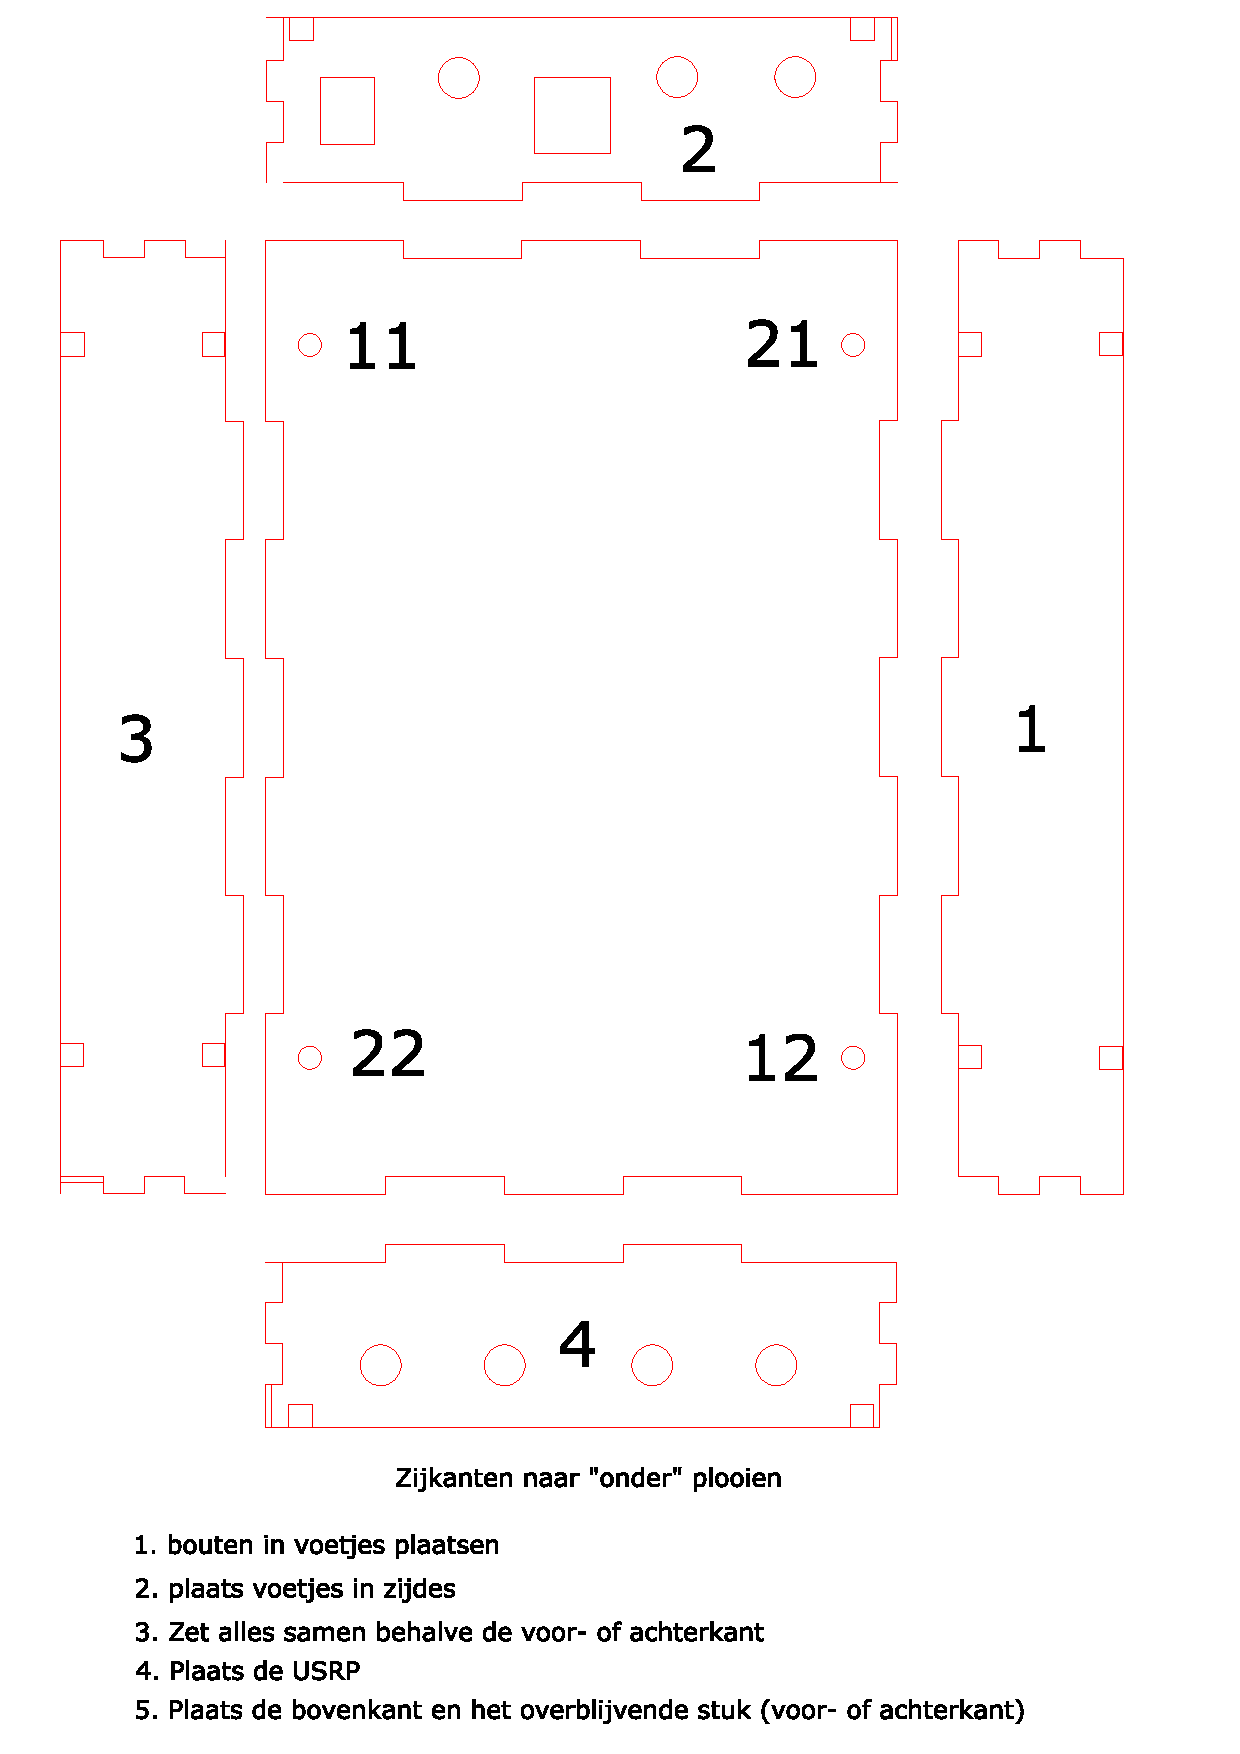
\includegraphics[clip, trim=0mm 50mm 0mm 0mm, width=0.8\textwidth]{figs/assemble_case.pdf}\caption{Exploded view of the B210 casing. The numbers indicate which component should be placed where.}\label{fig:b210-case}
\end{figure}

\section{Getting started with GNU Radio}


Read~\cref{sec:sdrgnur} thoroughly before installing \gls{grc}.

Follow the following sections on \url{https://wiki.gnuradio.org/index.php?title=Tutorials}:
\begin{itemize}
    \item Beginner Tutorials
    \begin{itemize}
         \item Introducing GNU Radio
         \item Flowgraph Fundamentals
    \end{itemize}
    \item Intermediate/Advanced Tutorials
    \begin{itemize}
        \item Miscellaneous
        \begin{itemize}
            %\item Understanding a Flowgraph's Python Code
            \item Using GNU Radio With SDRs
            \item IQ and Complex Signals
            \item Understanding Sample Rate
        \end{itemize}


    \end{itemize}
   
\end{itemize}
It is imperative for the remainder of the lab sessions that you will carefully and thoroughly go through each of those tutorials. Additionally, follow the introduction tutorial on complex signals if you are not yet familiar with concepts such as complex \gls{bb} and pass band (\url{https://wiki.gnuradio.org/index.php?title=IQ_Complex_Tutorial}). 



\section{Getting to know OFDM}
Start by reading~\cref{sec:basic} with a special focus on Section~\ref{sec:ofdm-laymen},~\ref{sec:ofdm-overview},~\ref{ss:equ},~\ref{sec:cohmod}.
After this the building blocks of \gls{ofdm} should be clear. 

After completing this, consult the \textit{Basic OFDM Tutorial} of GR (\url{https://wiki.gnuradio.org/index.php?title=Basic_OFDM_Tutorial}). Create the \textit{Example loopback flowgraph}. After this, and grasping all the required knowledge to thoroughly understand this flowgraph, run this flowgraph and ask your teaching assistant to evaluate your progress.


